\documentclass[german,10pt]{book}      
\usepackage{makeidx}
\usepackage{babel}            % Sprachunterstuetzung
\usepackage{amsmath}          % AMS "Grundpaket"
\usepackage{amssymb,amsfonts,amsthm,amscd} 
\usepackage{mathrsfs}
\usepackage{rotating}
\usepackage{sidecap}
\usepackage{graphicx}
\usepackage{color}
\usepackage{fancybox}
\usepackage{tikz}
\usetikzlibrary{arrows,snakes,backgrounds}
\usepackage{hyperref}
\hypersetup{colorlinks=true,
                    linkcolor=blue,
                    filecolor=magenta,
                    urlcolor=cyan,
                    pdftitle={Overleaf Example},
                    pdfpagemode=FullScreen,}
%\newcommand{\hyperref}[1]{\ref{#1}}
%
\definecolor{Gray}{gray}{0.80}
\DeclareMathSymbol{,}{\mathord}{letters}{"3B}
%
\newcounter{num}
\renewcommand{\thenum}{\arabic{num}}
\newenvironment{anmerkungen}
   {\begin{list}{(\thenum)}{%
   \usecounter{num}%
   \leftmargin0pt
   \itemindent5pt
   \topsep0pt
   \labelwidth0pt}%
   }{\end{list}}
%
\renewcommand{\arraystretch}{1.15}                % in Formeln und Tabellen   
\renewcommand{\baselinestretch}{1.15}                 % 1.15 facher
                                                      % Zeilenabst.
\newcommand{\Anmerkung}[1]{{\begin{footnotesize}#1 \end{footnotesize}}\\[0.2cm]}
\newcommand{\comment}[1]{}
\setlength{\parindent}{0em}           % Nicht einruecken am Anfang der Zeile 

\setlength{\textwidth}{15.4cm}
\setlength{\textheight}{23.0cm}
\setlength{\oddsidemargin}{1.0mm} 
\setlength{\evensidemargin}{-6.5mm}
\setlength{\topmargin}{-10mm} 
\setlength{\headheight}{0mm}
\newcommand{\identity}{{\bf 1}}
%
\newcommand{\vs}{\vspace{0.3cm}}
\newcommand{\noi}{\noindent}
\newcommand{\leer}{}

\newcommand{\engl}[1]{[\textit{#1}]}
\parindent 1.2cm
\sloppy

         \begin{document}  \setcounter{chapter}{6}


\chapter{Grundlagen der ART}
% Kap x
\label{chap_ART}

Einige der Kurztexte im Rahmen dieser Reihe beziehen sich auf die Allgemeine
Relativit\"atstheorie. Es gibt einen Kurztext zu Schwarzen L\"ochern, einen
Kurztext zu Gravitationswellen und einen Kurztext zu Kosmologischen Modellen.
In allen F\"allen handelt es sich um spezielle L\"osungen der Einstein'schen
Feldgleichungen. Daher ist es sinnvoll, eine kurze Einf\"uhrung in die
Ideen und Konzepte der Allgemeinen Relativit\"atstheorie zu geben. Sie
bilden die Grundlagen der anderen Kapitel zur ART und tragen so hoffentlich zum besseren
Verst\"andnis bei. 

Der mathematische Formalismus der Allgemeinen Relativit\"atstheorie ist die
Differentialgeometrie. Ausgehend vom Konzept einer Mannigfaltigkeit mit einer
symmetrischen Bilinearform (in der Physik spricht man von einer Metrik, obwohl
diese Bilinearform nicht positiv definit ist) gelangt man schlie\ss lich zum
Kr\"ummungstensor und seinen Verk\"urzungen, dem Ricci-Tensor und dem
Kr\"ummungsskalar, die in die Einstein'schen Gleichungen eingehen. Bis zu einem gewissen
Grad kann man diese Beitr\"age veranschaulichen, was in den kommenden Abschnitten
geschehen soll. Die Einstein'schen Gleichungen lassen sich zwar nicht herleiten, aber
sie folgen aus einfachen Annahmen. 

Die L\"osung der Einstein'schen Gleichungen besteht in einem tensorwertigen Feld
(eine symmetrische $4\times 4$ Matrix an jedem Punkt der Raumzeit), $g_{\mu \nu}(x)$,
dem sogenannten metrischen Feldtensor.
Dieses Feld kann als ein vom Ort abh\"angiger Ma\ss stab auf einer Karte interpretiert
werden und gibt Aufschluss \"uber die lokalen geometrischen Eigenschaften der
Raumzeit. Daher wird in diesem Kapitel auch angedeutet, wie man solche Karten mit
einer Metrik interpretieren kann. 

\section{Vorbemerkungen und Definitionen}

In der Allgemeinen Relativit\"atstheorie betrachten wir eine 4-dimensionale Raumzeit mit einer Zeit- und 
drei Raumdimensionen.
Die Elemente der Raumzeit bezeichnen wir als \textit{Ereignisse}: Dabei handelt es sich um
zeitlich und r\"aumlich lokalisierte physikalische Prozesse wie beispielsweise das
Ein- oder Ausschalten einer punktf\"ormigen Lichtquelle, die Zeigerstellung einer Uhr in Richtung
einer bestimmten Zahl, das Zusammentreffen zweier Weltlinien von Objekten, etc. 
Jedes Ereignis kann durch die Angabe von vier Zahlen, die durch ein lokales Koordinatensystem
festgelegt sind, charakterisiert werden: Eine dieser Koordinaten bezieht sich auf den Zeitpunkt,
die anderen drei Koordinaten dienen der r\"aumlichen Festlegung des Ereignisses. In diesem
Kapitel verwenden wir oft euklidische R\"aume zur Veranschaulichung von geometrischen
Eigenschaften oder auch 2- und 3-dimensionale Raumzeiten zur Vereinfachung der Darstellungen. 

\begin{SCfigure}[30][htb]
\begin{tikzpicture}
\draw (0,0.5) node{~};
\draw[->] (0.5,3) -- (5.5,3);
\draw[->] (3,0) -- (3,6);
\draw[->] (2,2.35) -- (3.8,3.5);
\draw (1,1) -- (5,5);
\draw (1,5) -- (5,1);
\draw (3,5) ellipse (2 and 0.3);
\draw (3,1) ellipse (2 and 0.3);
\draw (3,2) ellipse (1 and 0.15);
\draw (3,4) ellipse (1 and 0.15);
\filldraw[fill=black!100] (3,3) circle (0.05);
\filldraw[fill=black!100] (3.7,3.9) circle (0.05);
\filldraw[fill=black!100] (2,0.75) circle (0.05);
\filldraw[fill=black!100] (4,3.3) circle (0.05);
\filldraw[fill=black!100] (2.5,4.4) circle (0.05);
\filldraw[fill=black!100] (3.5,1.5) circle (0.05);
\draw (2.88,2.8) node {${\scriptstyle A}$};
\draw (3.5,4) node {${\scriptstyle L_1}$};
\draw (2.25,0.85) node {${\scriptstyle L_2}$};
\draw (4.2,3.3) node {${\scriptstyle C}$};
\draw (2.7,4.4) node {${\scriptstyle Z}$};
\draw (3.7,1.5) node {${\scriptstyle V}$};
\draw (3.15,5.8) node {${\scriptstyle t}$};
\draw (5.6,2.9) node {${\scriptstyle x}$};
\draw (3.9,3.6) node {${\scriptstyle y}$};
\end{tikzpicture}
\caption{\label{fig_ART_Lichtkegel}%
Der Lichtkegel zu einem Ereignis $A$. Das Ereignis $L_1$ liegt auf dem zuk\"uftigen
Teil des Lichtkegels von $A$, das Ereignis $L_2$ liegt auf dem vergangenen Teil des Lichtkegels von $A$.
$C$ liegt im kausalen Komplement zu $A$. Ereignis $Z$ liegt innerhalb des Zukunftslichtkegels und
kann von $A$ beeinflusst werden, Ereignis $V$ liegt innerhalb des Vergangenheitslichtkegels
und kann Ereignis $A$ beeinflussen.}
\end{SCfigure}

Zu jedem Ereignis $A$ gibt es die zugeh\"orige (lokale) kausale Struktur (siehe Abb.\ \ref{fig_ART_Lichtkegel}). 
F\"ur jedes Ereignis $A$ wird die Menge aller Ereignisse in drei Klassen eingeteilt: (1) Die Menge aller
zuk\"uftigen Ereignisse $\{Z\}_A$, die ausgehend von $A$ von der Weltlinie eines Objekts erreicht
und somit von dem Ereignis $A$ beeinflusst werden k\"onnen, (2) die Menge aller Ereignisse in der
Vergangenheit relativ zu $A$, also alle Ereignisse, von denen ausgehend ein Objekt das Ereignis
$A$ erreichen und somit beeinflussen kann, und (3) das kausale Komplement von $A$, das sind alle
Ereignisse $C$, die weder von $A$ beeinflusst werden k\"onnen noch $A$ beeinflussen k\"onnen.
Die Mantellinie zwischen den Ereignissen, die eine kausale Beziehung zu $A$ haben und dem
kausalen Komplement von $A$ bezeichnet man als Lichtkegel und die Ereignisse auf dem Lichtkegel
als lichtartige Ereignisse. Der Lichtkegel besteht aus den Ereignissen $\{L\}_A$, die von einem Lichtblitz, 
der von Ereignis $A$ ausgeht, getroffen werden,
sowie aus den Ereignissen, von denen ausgehend ein Lichtblitz das Ereignis $A$ trifft.
Die Einteilung der Ereignisse in Zukunft, Vergangenheit und kausales Komplement relativ zu
einem Ereignis $A$ ist unabh\"angig von einem Beobachter oder Bezugssystem.\footnote{Manchmal
versteht man unter der Lichtkegelstruktur auch die durch die hier beschriebene kausale Struktur  
induzierte Struktur auf dem Tangentialraum zu einem Ereignis - dem Raum der Geschwindigkeiten, 
mit denen Wege, insbesondere Weltlinien, dieses Ereignis durchlaufen k\"onnen.}

Griechische Indizes $\mu, \nu, ...$ nehmen
die Werte 0,1,2,3 an, wobei sich 0 auf die Zeitkoordinate und 1,2,3 auf die r\"aumlichen
Koordinaten beziehen. Lateinische Indizes $i,j,k,...$ bezeichnen meist die rein r\"aumlichen
Koordinaten und nehmen dann die Werte 1,2,3 an. Au\ss erdem verwende ich die Einstein'sche
Summenkonvention: \"Uber doppelt auftretende Indizes auf einer Seite einer Gleichung - ein Index
oben, der andere unten - ist zu summieren. Steht derselbe Index auf den beiden Seiten einer
Gleichung, muss er in beiden F\"allen entweder oben oder unten stehen.
Ein Index sollte (in einer
kovarianten Notation) nie \"ofter als zweimal auftreten, er sollte auf derselben Seite einer
Gleichung nie beide Male oben oder unten stehen und er sollte auf verschiedenen Seiten einer
Gleichung nie an verschiedenen Positionen (einmal oben und einmal unten) stehen. 
In solchen F\"allen hat man meist einen Fehler gemacht. Vierervektoren werden normal
geschrieben ($x$), die r\"aumlichen 3-dimensionalen Anteile dieser Vektoren in boldface
($\pmb{x}$). Die Vorzeichen in der Minkowski-Metrik (und allgemein der Metriken in der ART)
seinen $\eta_{\mu \nu}={\rm diag}(1,-1,-1,-1)$, sodass zeitartige Vektoren $x$ eine positive
\glqq L\"ange\grqq\ haben: $\eta_{\mu \nu}x^\mu x^\nu = (x^0)^2 - (\pmb{x})^2 > 0$. 

Da es sich nicht um eine euklidische Metrik handelt, muss man zwischen den Komponenten
von Vektoren, die oben stehen, und den Komponenten von dualen Vektoren, die unten stehen,
unterscheiden. Letztendlich entscheidet die Art, wie sich ein Satz von Gr\"o\ss en unter
einer Koordinatentransformation \"andert, ob es sich um ko- (Indizes stehen oben) oder 
kontravariante (Indizes stehen unten) Gr\"o\ss en handelt. Mit der Metrik kann ein Index
rauf oder runter gezogen werden:
\begin{equation}
                 A^{i} g_{ij} = A_j \hspace{1cm}    A_i g^{ij} = A^j \, .
\end{equation}
Die beiden Bilinearformen $g^{ij}$ und $g_{ij}$ sind invers zueinander:
\begin{equation}
                 g^{ik} g_{kj} = \delta^i_j  \, .
\end{equation}



\section{Elementare Differentialgeometrie - von der Metrik zur Kr\"ummung}

In der Differentialgeometrie betrachtet man meist sogenannte Riemann'sche Mannigfaltigkeiten,
bei denen an jedem Punkt eine positiv definite Metrik vorgegeben ist, die lokal eine Abstandsfunktion zwischen
Punkten definiert. In der Allgemeinen Relativit\"atstheorie handelt es sich jedoch streng genommen
nicht um eine Metrik sondern nur um eine nicht entartete, symmetrische Bilinearform (die Positivit\"at
fehlt). Der Grund ist die Signatur der Biliniearform, die schon von der Minkowski-Metrik
$\eta_{\mu \nu}={\rm diag}(1,-1,-1,-1)$ bekannt ist. \glqq Nicht entartet\grqq\ bedeutet, dass es
keine von null verschiedenen Vektoren gibt, deren Produkt (gebildet mit der Bilinearform) mit allen
anderen Vektoren verschwindet. Trotz dieser Eigenschaften ist in der Physik der Begriff
\glqq Metrik\grqq\ verbreitet, gelegentlich spricht man auch von einer Pseudometrik und
Pseudo-Riemann'schen Mannigfaltigkeiten. Gl\"ucklicherweise unterscheidet sich die Differentialgeometrie
der Riemann'schen Mannigfaltigkeiten und der Pseudo-Riemann'schen Mannigfaltigkeiten in vielerlei
Hinsicht kaum, sodass die differentialgeometrischen Grundlagen anhand der Riemann'schen
Geometrie veranschaulicht werden k\"onnen. 

Die Allgemeine Relativit\"atstheorie ist eine geometrische Theorie der Raumzeit. Um Geometrie
betreiben zu k\"onnen, muss man zun\"achst festlegen, auf was f\"ur Objekten man Geometrie
betreiben m\"ochte - das sind in der Differentialgeometrie sogenannte Mannigfaltigkeiten - und
man muss wissen, wie man die L\"ange von Wegen bestimmen kann bzw.\ wie man f\"ur 
infinitesimal benachbarte Punkte deren Abstand bestimmen kann (dann kann man die L\"ange
von Wegen durch Integration \"uber infinitesimale Abschnitte bestimmen). Die wichtigsten Schritte von
der Mannigfaltigkeit bis zum sogenannten Kr\"ummungstensor seien im Folgenden kurz skizziert.

\subsection{Mannigfaltigkeiten, Karten und Atlanten}

Eine Mannigfaltigkeit ist im Wesentlichen ein topologischer Raum, bei dem es zu jedem Punkt
eine Umgebung gibt, f\"ur die eine bijektive Abbildung in eine Umgebung im $\mathbb{R}^n$ definiert ist. Eine
solche Umgebung mit dieser Abbildung bezeichnet man als Karte, und die Menge aller Karten
als einen Atlas. Diese Terminologie darf man w\"ortlich nehmen: Eine
Mannigfaltigkeit ist definiert durch den Atlas ihrer Karten. Wenn zwei Karten Ausschnitte desselben
Gebiets der Mannigfaltigkeit darstellen, sollen diese Gebiete nat\"urlich isomorph sein (wenn man in
einem Weltatlas zwei Karten findet, auf denen Deutschland dargestellt ist, sollten die beiden
dargestellten Gebiete in ihren topologischen Eigenschaften gleich sein). Man verlangt von diesen
Abbildungen von einer Karte zu einer anderen Karte mindestens, dass sie differenzierbar sind, meist
verlangt man sogar, dass sie unendlich oft differenzierbar sind. Man sagt dann, dass der Atlas mit
seinen Karten auf der Mannigfaltigkeit eine differenzierbare Struktur definiert. W\"ahrend man auf der
Mannigfaltigkeit selbst zun\"achst weder ableiten noch integrieren kann, ist dies auf den Karten
m\"oglich.

Da eine Karte unter anderem aus einer offenen Teilmenge des $\mathbb{R}^n$ besteht, kann man
in diesem Gebiet ein Koordinatensystem w\"ahlen. \"Uber die bijektive Kartenabbildung kann dieses
Koordinatensystem auf ein lokales Koordinatensystem auf der Mannigfaltigkeit abgebildet werden. Verschiedene
Karten definierten somit verschiedene Koordinatensysteme auf der Mannigfaltigkeit und die Kunst
besteht oftmals darin, zu einem gegebenen Ausschnitt einer Mannigfaltigkeit eine m\"oglichst intuitive oder
einfache Karte mit ihrem zugeh\"origen Koordinatensystem zu finden.

Karten haben oft die Eigenschaft, dass sie einen Rand haben, an dem die Karte bzw.\ ihre
Koordinaten \glqq singul\"ar\grqq\
werden. Ein Beispiel sind typische Weltkarten, die am Nord- und S\"udpol singul\"ar sind: Sowohl
der Nordpol als auch der S\"udpol erstrecken sich \"uber den gesamten oberen bzw.\ unteren Rand der
Karte, obwohl es sich dabei auf der Weltkugel um regul\"are Punkte handelt. Ein anderes Beispiel ist die 
Karte der Welt (also eine zweidimensionale Darstellung auf einer flachen Ebene), die
man erh\"alt, wenn man aus einem gro\ss en Abstand auf die Welt blickt. Diese Karte ist am Rand
wieder singul\"ar in dem Sinne, dass dort die Gebiete in radialer Richtung
unendlich dicht zusammenzur\"ucken scheinen (siehe z.B.\ Abb.\ \ref{fig_ART_Tissot}, links).
Au\ss erdem h\"ort die Karte dort auf, obwohl in Wirklichkeit dort keine besonderen Punkte
liegen. Solche Singularit\"aten bezeichnet man als Koordinatensingularit\"aten (manchmal auch als 
Kartensingularit\"aten): Die Darstellung auf der Karte
ist dort nicht mehr stetig und bijektiv, obwohl es sich in Wirklichkeit um keine besonderen Punkte
handelt. Bei dem Horizont der Schwarzschild-L\"osung handelt es sich um eine solche Koordinatensingularit\"at,
wohingegen die Singularit\"at bei $r=0$ physikalisch ist; dort wird die Kr\"ummung unendlich.

\subsection{Tangentialr\"aume}

Man stellt sich eine Tangentialebene an eine gekr\"ummte Fl\"ache gerne als einen euklidische Ebene vor, die
an einem Punkt die Fl\"ache gerade ber\"uhrt, ohne sie zu schneiden. Diese Vorstellung geht
von einer Einbettung aus (siehe Abschnitt \ref{sec_ART_Grundzuege})
und die Tangentialebene ist dann in denselben Raum eingebettet wie auch
die Fl\"ache. Diese Vorstellung ist etwas irref\"uhrend, da beispielsweise eine 2-dimensionale
Fl\"ache an jedem Punkt eine 2-dimensionalen Tangentialebene hat und die Fl\"ache mit ihren
Tangentialebenen 4-dimensional ist. Au\ss erdem f\"uhrt es oft zu Fehlvorstellungen, wenn man die
Tangentialebenen an eine Ebene betrachtet: Man tendiert dazu, die beiden als \glqq dasselbe\grqq\ 
anzusehen. 

Eine etwas bessere Vorstellung eines Tangentialvektors ist die Vorstellung einer Geschwindigkeit $v$,
die eine Bahnkurve $x(s)$ (hier ist eine Bahnkurve definiert als ein parametrisierter Weg, d.h.\ als eine
Abbildung von einem 1-dimensionalen Parameterraum in die Mannigfaltigkeit) 
in einem Punkt $p$ haben kann. Man definiert zwei Bahnkurven, die sich in einem
Punkt $p$ treffen, als \"aquivalent, wenn sie in diesem Punkt dieselbe Geschwindigkeit haben. Wir k\"onnen
zwar auf der Mannigfaltigkeit selbst keine Ableitungen bilden (sie ist nur ein topologischer Raum), aber wir
k\"onnen auf den Karten ableiten und wenn diese Karten in einem Punkt regul\"ar sind, sind zwei
Wege, die in obigem Sinne in einer Karte \"aquivalent sind, in allen Karten \"aquivalent. Insofern handelt
es sich um eine Eigenschaft der Wege auf der Mannigfaltigkeit. Mit der Definition einer Addition und einer
skalaren Multiplikation auf diesen \"Aquivalentklassen von Wegen - dem Raum der Geschwindigkeiten - wird 
dieser Raum zu einem
Vektorraum. Diesen Vektorraum bezeichnet man als den Tangentialraum an eine Fl\"ache im Punkte $p$. 
Diese Definition l\"asst sich auch sofort auf beliebige Mannigfaltigkeiten erweitern und \"ahnlich
wie bei eingebetteten R\"aumen hat der Tangentialraum in einem Punkte $p$ dieselbe Dimension wie
die Mannigfaltigkeit selbst. 

Die kausale Struktur der ART, die wir lokal f\"ur eine Raumzeit definiert haben, \"ubertr\"agt sich auf den
Tangentialraum. Eine physikalische Weltlinie ist eine parametrisiert Kurve in der Raumzeit, bei der an jedem
Punkt der Geschwindigkeitsvektor zeitartig ist, also innerhalb des positiven Lichtkegels liegt. F\"ur
masselose Objekten wird die Definition der Weltlinie auch auf lichtartige Weltlinien (mit
lichtartigen Tangentialvektoren) erweitert. 
    
\subsection{Der metrische Feldtensor}

Zur Festlegung der geometrischen Eigenschaften einer Mannigfaltigkeit muss
f\"ur jede Karte und jeden Punkt auf dieser
Karte lokal angegeben werden, welchen Abstand zwei eng benachbarte Punkte der Karte
in Wirklichkeit haben. Dies \"ubernimmt bei einer Landkarte der Ma\ss stabsfaktor, der allerdings
in $x$- und $y$-Richtung verschieden sein kann; au\ss erdem kann es sein, dass
in Wirklichkeit orthogonale Linien auf einer Karte nicht unter $90^\circ$ dargestellt werden. Auch diese
Information muss vorhanden sein. In zwei Dimensionen reichen daf\"ur drei Zahlen, die in Form einer
symmetrischen $2\times2$-Matrix $g_{ij}$ zusammengefasst werden. Diese drei Zahlen geben an, wie
ein Kreis vom Radius $r$ \glqq in der Wirklichkeit\grqq\ auf der Karte wiedergegeben wird: Dort
erscheint dieser Kreis im Allgemeinen als Ellipse und man muss die beiden Halbachsen sowie einen Winkel f\"ur die
Orientierung dieser Ellipse kennen. (Siehe Kapitel \ref{chap_Metrik}, wo die Analogie zwischen dem
metrischen Feldtensor und Ma\ss st\"aben bei Landkarten ausf\"uhrlicher behandelt wird.)

Seien $p$ und $p'$ zwei eng benachtbarte Punkte auf der Mannigfaltigkeit und $\{x^i\}$ bzw.\ $\{x^{\prime i}\}$
ihre Koordinaten in einer Karte. Au\ss erdem sei ${\rm d}x^i=x^{\prime i}-x^i$ die Differenz der $i$-ten
Koordinate f\"ur die beiden Punkte. \glqq In Wirklichkeit\grqq\ sollen die beiden Punkte den Abstand
${\rm d}s$ haben. Dann gilt 
\begin{equation}
\label{eq_ART_Metrik}
              {\rm d}s^2 = g(x)_{ij}\, {\rm d} x^i\, {\rm d} x^j  \hspace{2cm} \mbox{(Einstein'sche Summenkonvention!)}
\end{equation}
Diese Gleichung beschreibt in der Karte eine Ellipse, wobei die Eigenwerte von $g$ der gro\ss en und kleinen
Halbachse entsprechen und die zugeh\"origen Eigenr\"aume (die Hauptachsen) die Orientierung der Ellipse. 
Die Angabe dieser Ellipsen in einer Karte bezeichnet man auch als Tissot-Indikatrix. 
Man kann sich vorstellen, dass man um $p$ bzw.\ $p'$
(das sollte in f\"uhrender Ordnung keine Rolle spielen, da die beiden Punkte infinitesimal benachbart sind)
einen Kreis vorgibt, sodass einer der Punkte im Mittelpunkt ist und der andere auf dem Kreisrand. Der Radius
des Kreises ist dann ${\rm d}s$. In einer Karte wird dieser Kreis durch eine Ellipse dargestellt, deren Parameter
(Orientierung und Halbachsen) die Hauptachsen und Eigenwerte von $g_{ij}(x)$ sind. Au\ss erdem h\"angt die
Matrix $g$ vom Punkte $x$ ab, d.h., die Ma\ss st\"abe k\"onnen an jedem Punkt anders sein, sollten
aber stetig von $x$ abh\"angen (siehe Abb.\ \ref{fig_ART_Tissot}).

\begin{figure}[htb]
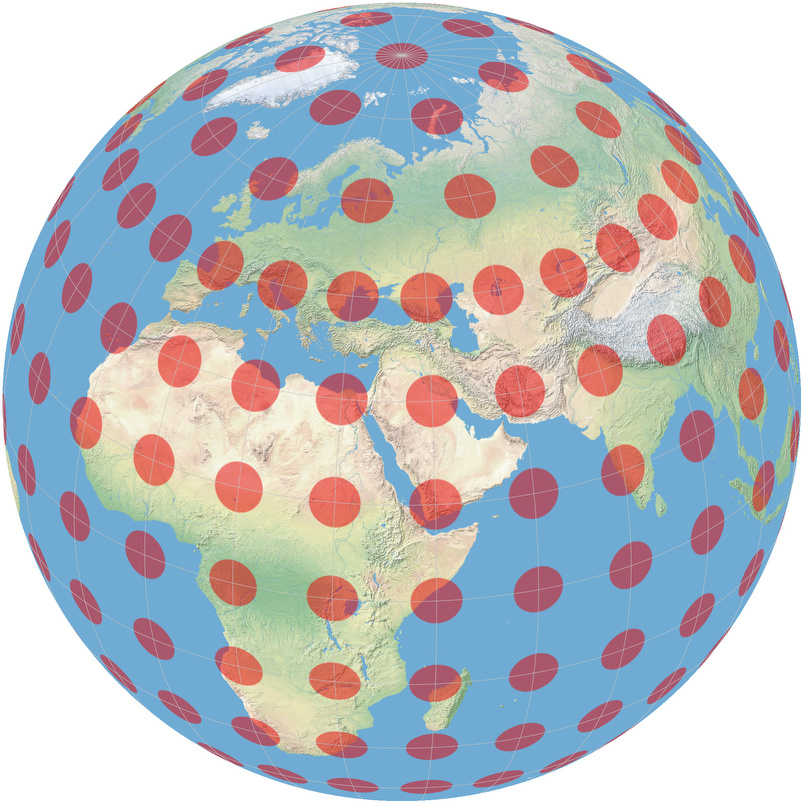
\includegraphics[scale=0.18]{./Bilder/Tissot_orthographic.jpg}
\hfill
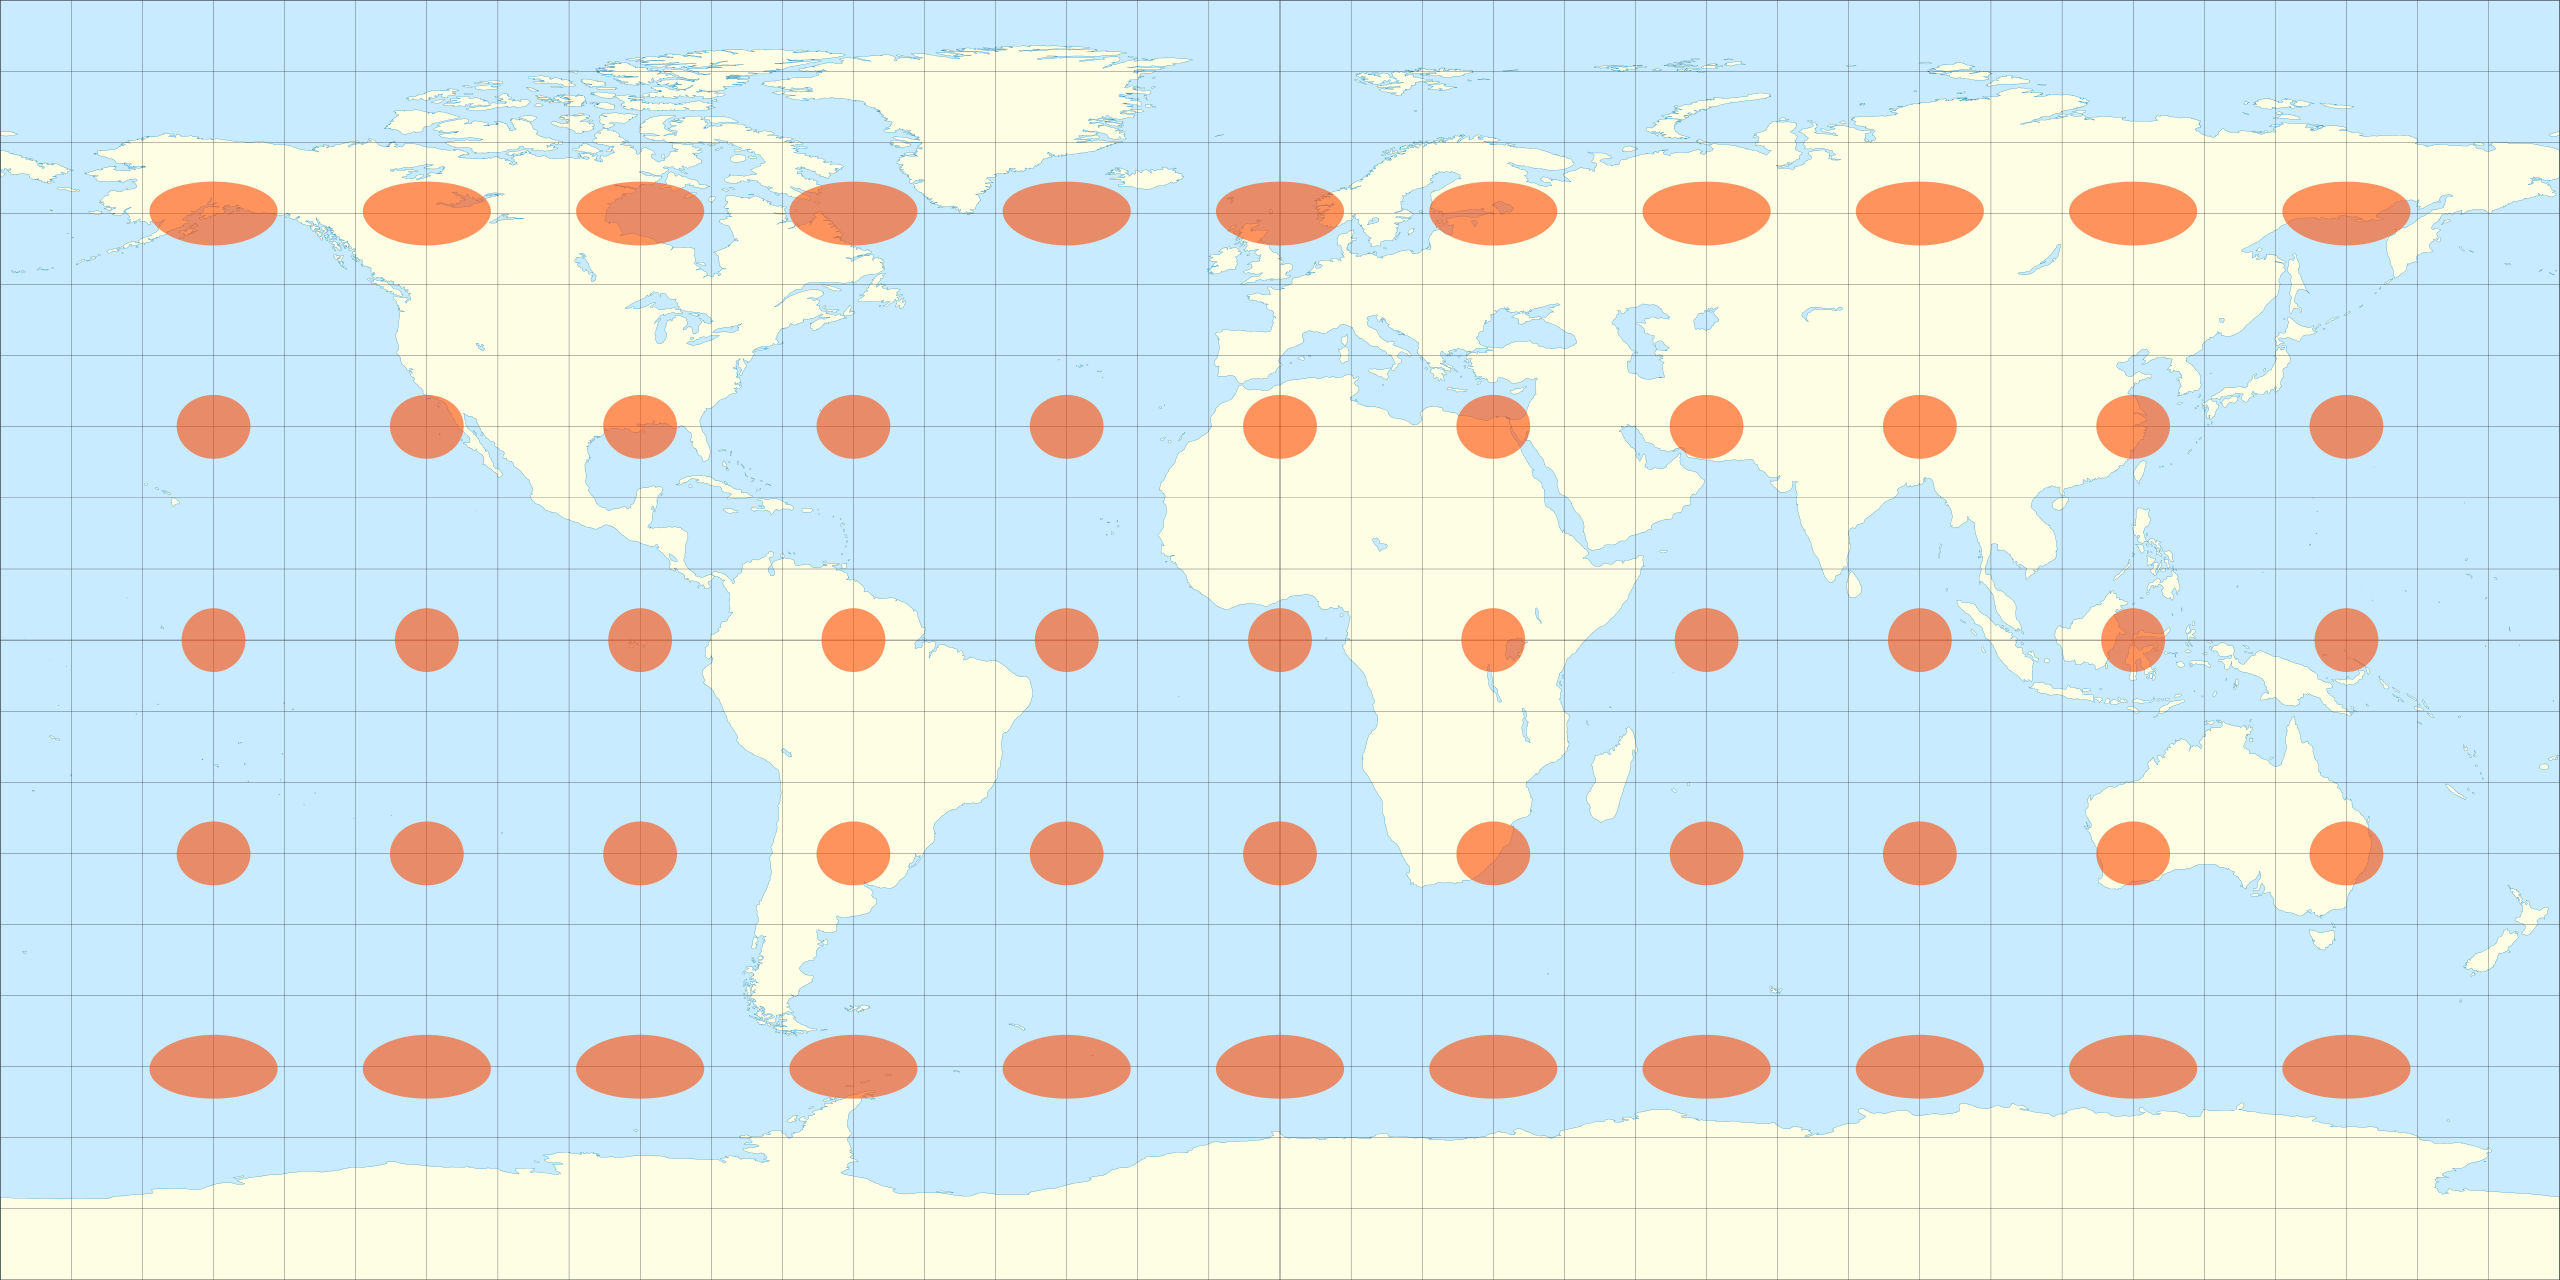
\includegraphics[scale=0.11]{./Bilder/Tissot_rectangle.png}
\caption{\label{fig_ART_Tissot}%
Zwei Darstellungen einer Kugeloberfl\"ache mit Tissot-Indikatrix. (links) Hier kann man sich
eine dreidimensionale Einbettung der Kugel vorstellen mit eingezeichneten Kreisen (aus \cite{Tissot}). 
(rechts) Eine orthogonale Rechteckdarstellung der Kugeloberfl\"ache mit Tissot-Ellipsen
(aus \cite{WikiTissot}).} 
\end{figure}

In mehr als zwei Dimensionen wird aus dem Kreis die $d-1$-dimensionale Kugeloberfl\"ache einer 
$d$-dimensionalen Kugel und die Ellipse wird zu einem entsprechenden Ellipsoid. In der ART wird der Kreis
zu zwei Doppelhyperbeln - eine r\"aumliche im kausalen Komplement und eine zeitliche. In mehr als zwei
Dimensionen wird die zeitliche Hyperbel ein mehrdimensionaler Hyperboloid. Die r\"aumlichen Hyperbeln sind um
die Zeitachse zu drehen.   

\begin{figure}[htb]
\mbox{~}~
\begin{tikzpicture}[scale=0.9]
\draw[thick] (4,3) circle (0.4);
\draw[thick] (4,3) circle (0.8);
\draw[thick] (4,3) circle (1.2);
\draw[thick] (4,3) circle (1.6);
\draw[thick] (4,3) circle (2.0);
\draw[thick] (4,3) circle (2.4);
\draw[thick] (4,3) circle (2.8);
\draw[thick] (4,3) circle (3.2);
\filldraw[fill=black!100] (4,3) circle (0.06);
\filldraw[fill=black!100] (5.2,4.6) circle (0.06);
\draw (4.15,2.95) node{${\scriptstyle A}$};
\draw (5.4,4.65) node{${\scriptstyle B}$};
\draw (3.86,3) node{${\scriptstyle 0}$};
\draw (3.48,3) node{${\scriptstyle 1}$};
\draw (3.08,3) node{${\scriptstyle 2}$};
\draw (2.68,3) node{${\scriptstyle 3}$};
\draw (2.28,3) node{${\scriptstyle 4}$};
\draw (1.88,3) node{${\scriptstyle 5}$};
\draw (1.48,3) node{${\scriptstyle 6}$};
\draw (1.08,3) node{${\scriptstyle 7}$};
\draw (0.68,3) node{${\scriptstyle 8}$};
%\filldraw[fill=black!100] (13,3) circle (0.04);
\end{tikzpicture}
\hspace{1.0cm}
\begin{tikzpicture}[scale=0.9]
\draw[thick] (0,6) -- (6,0); 
\draw[thick] (0,0) -- (6,6); 
\filldraw[fill=black!100] (3,3) circle (0.06);
\filldraw[fill=black!100] (4.2,4.6) circle (0.06);
\draw (3.19,3) node{${\scriptstyle A}$};
\draw (4,4.65) node{${\scriptstyle B}$};
\draw (2.85,3) node{${\scriptstyle 0}$};
\draw (3,3.53) node{${\scriptstyle 1}$};
\draw (3,3.93) node{${\scriptstyle 2}$};
\draw (3,4.26) node{${\scriptstyle 3}$};
\draw (3,4.64) node{${\scriptstyle 4}$};
\draw (3,5.0) node{${\scriptstyle 5}$};
\draw (3,5.4) node{${\scriptstyle 6}$};
\draw (3,5.8) node{${\scriptstyle 7}$};
%   oben
\draw[thick] (0.05,6) .. controls (2.75,3.4) .. (3,3.4) .. controls (3.25,3.4) ..  (5.95,6); 
\draw[thick] (0.1,6) .. controls (2.5,3.8) .. (3,3.8) .. controls (3.5,3.8) .. (5.9,6); 
\draw[thick] (0.2,6) .. controls (2.9,3.5) and (3.1,3.5) .. (5.8,6); 
\draw[thick] (0.3,6) .. controls (2.7,4.0) and (3.3,4.0) .. (5.7,6); 
\draw[thick] (0.4,6) .. controls (2.6,4.5) and (3.4,4.5) .. (5.6,6); 
\draw[thick] (0.7,6) .. controls (2.5,5.0) and (3.5,5.0) .. (5.3,6); 
\draw[thick] (1,6) .. controls (2.4,5.5) and (3.6,5.5) .. (5,6); 
% unten
\draw[thick] (0.05,0) .. controls (2.75,2.6) .. (3,2.6) .. controls (3.25,2.6) ..  (5.95,0); 
\draw[thick] (0.1,0) .. controls (2.5,2.2) .. (3,2.2) .. controls (3.5,2.2) .. (5.9,0); 
\draw[thick] (0.2,0) .. controls (2.9,2.5) and (3.1,2.5) .. (5.8,0); 
\draw[thick] (0.3,0) .. controls (2.7,2.0) and (3.3,2.0) .. (5.7,0); 
\draw[thick] (0.4,0) .. controls (2.6,1.5) and (3.4,1.5) .. (5.6,0); 
\draw[thick] (0.7,0) .. controls (2.5,1.0) and (3.5,1.0) .. (5.3,0); 
\draw[thick] (1,0) .. controls (2.4,0.5) and (3.6,0.5) .. (5,0); 
%   rechts
\draw[thick] (6,0.05) .. controls (3.4,2.75) .. (3.4,3) .. controls (3.4,3.25) ..  (6,5.95); 
\draw[thick] (6,0.1) .. controls (3.8,2.5) .. (3.8,3) .. controls (3.8,3.5) .. (6,5.9); 
\draw[thick] (6,0.2) .. controls (3.5,2.9) and (3.5,3.1) .. (6,5.8); 
\draw[thick] (6,0.3) .. controls (4,2.7) and (4,3.3) .. (6,5.7); 
\draw[thick] (6,0.4) .. controls (4.5,2.6) and (4.5,3.4) .. (6,5.6); 
\draw[thick] (6,0.7) .. controls (5.0,2.5) and (5.0,3.5) .. (6,5.3); 
\draw[thick] (6,1) .. controls (5.5,2.4) and (5.5,3.6) .. (6,5); 
%   links
\draw[thick] (0,0.05) .. controls (2.6,2.75) .. (2.6,3) .. controls (2.6,3.25) ..  (0,5.95); 
\draw[thick] (0,0.1) .. controls (2.2,2.5) .. (2.2,3) .. controls (2.2,3.5) .. (0,5.9); 
\draw[thick] (0,0.2) .. controls (2.5,2.9) and (2.5,3.1) .. (0,5.8); 
\draw[thick] (0,0.3) .. controls (2.0,2.7) and (2.0,3.3) .. (0,5.7); 
\draw[thick] (0,0.4) .. controls (1.5,2.6) and (1.5,3.4) .. (0,5.6); 
\draw[thick] (0,0.7) .. controls (1.0,2.5) and (1.0,3.5) .. (0,5.3); 
\draw[thick] (0,1) .. controls (0.5,2.4) and (0.5,3.6) .. (0,5); 
\end{tikzpicture}
\caption{\label{fig_ART_Schablone}%
(links) Im der euklidischen Ebene bilden Punkten mit einem festen Abstand zu einem vorgegebenen Punkt Kreise.
Die Punkte $A$ und $B$ im euklidischen Raum (links) haben einen Abstand 5: $A$ liegt im Zentrum und 
$B$ auf dem Kreis mit der Markierung $5$. 
(rechts) Im Minkowski-Raum bilden Punkte (Ereignisse) mit einem konstanten Abstand von einem
vorgegebenen Ereignis hyperbolische Kurven.
Die Punkte $A$ und $B$ auf der rechten Seite haben den
Abstand 3, da $B$ auf der Hyperbel mit der Markierung 3 liegt. In beiden F\"allen bezieht sich
\glqq Abstand\grqq\ immer auf die L\"ange einer geraden Verbindungslinie zwischen beiden Punkten.} 
\end{figure}


\subsection{Globale L\"angen und Geod\"aten}

Wir betrachten im Folgenden den metrischen Feldtensor $g_{\mu \nu}(x)$ als eine Gr\"o\ss e, die
es erlaubt, lokal Abst\"ande zwischen eng benachbarten Punkten anzugeben.  Kennen wir diese
Abst\"ande lokal, k\"onnen wir durch Integration entlang eines Weges auch die L\"ange beliebiger
Wege angeben, sowie Winkel, Fl\"achen und Volumina berechnen. F\"ur die L\"ange einer Weltlinie,
parametrisiert durch die Zeit $t$ in einem Bezugssystem, ergibt sich beispielsweise direkt aus
Gl.\ \ref{eq_ART_Metrik}:
\begin{equation}
\label{eq_ART_Laenge}
            L = \int_{t_0}^{t_1} \sqrt{g(x)_{ij}\, \frac{{\rm d} x^i}{{\rm d}t}\, \frac{{\rm d} x^j}{{\rm d}t}} {\rm d}t \, . 
\end{equation}
Damit k\"onnen wir die k\"urzesten
Verbindungslinien zwischen zwei Punkten bestimmen; solche Linien bezeichnet man als Geod\"aten. 

Streng genommen handelt es sich bei dem metrischen Tensor um eine Bilinearform im Tangentenraum 
an die Mannigfaltigkeit in einem Punkt. D.h., dieser Tensor ist auf Vektoren - Elemente des Tangentenraums - 
anzuwenden. Dies entspricht dem Skalarprodukt in krummlinigen Koordinaten. 
Jeder parametrisierte Weg hat jedoch in einem Punkt eine Tangente - seine Geschwindigkeit -
und das zeitliche Integral \"uber den Betrag der Geschwindigkeiten ergibt die zur\"uckgelegte Wegstrecke. 
Genau dies besagt Gl.\ \ref{eq_ART_Laenge}: Die Ableitung von $x$ nach $t$ ist die Geschwindigkeit und
die Wurzel in Gl.\ \ref{eq_ART_Laenge} ist der Betrag der Geschwindigkeit, der dann \"uber $t$ integriert wird.

\subsection{Parallelverschiebung von Vektoren - die Christoffel-Symbole}

F\"ur eine Geod\"ate k\"onnen wir angeben, wie ein Vektor entlang dieser Geod\"aten 
parallel zu verschieben ist: Seine L\"ange sowie sein Winkel relativ zur Tangente der
Geod\"aten bleiben gleich. Damit ist aber auch bekannt, wie man einen Vektor entlang eines
beliebigen Wegs parallel verschiebt: Man approximiert den Weg lokal durch Geod\"atenabschnitte,
bestimmt die Parallelverschiebung f\"ur diese und bildet das Integral. 

Allgemein bezeichnet man in der Differentialgeometrie eine Vorschrift, wie man Vektoren entlang
von Wegen parallel verschieben kann, als Zusammenhang (oder Zusammenhangsform). Ist eine
Metrik gegeben, kann man einen solchen Zusammenhang aus der Metrik berechnen. Diesen bezeichnet
man als Levi-Civita-Zusammenhang oder auch kovariante Ableitung. 

Sind zwei Vektorr\"aume derselben Dimension gegeben, kann man zun\"achst nicht sagen, welcher
Vektor in dem einen Vektorraum welchem Vektor in dem anderen Vektorraum entsprechen soll.
Dazu muss ein Isomorphismus zwischen diesen Vektorrr\"aumen definiert sein. Hat man mehrer
Vektorr\"aume, kann man Konsistenzbedingungen solcher Isomorphismen \"uberpr\"ufen:
Definieren die \"Aquivalenzen zwischen $V_1$ und $V_2$ sowie zwischen $V_2$ und $V_3$
dieselben \"Aquivalenz wie der Isomorphismus zwischen $V_1$ und $V_3$, etc. 
Ist das nicht der Fall, spricht man von einer Kr\"ummung. Bei Mannigfaltigkeiten mit ihren
Tangentialr\"aumen gibt es zwar eine sinnvolle Vorschrift, wie man solche Isomorphismen
zwischen verschiedenen Tangentialr\"aumen definiert, doch diese h\"angen im Allgemeinen
von einem Weg ab, entlang dem man diese Isomorphismen zun\"achst f\"ur infinitesimal
benachbarte Tangentialr\"aume definiert - dies macht der Zusammenhang - und dann kann
man diese entlang eines Weges aufintegrieren und erh\"alt einen sogenannten Paralleltransporter:
Einen vom Weg abh\"angigen Isomorphismus zwischen verschiedenen Tangentialr\"aumen.

Wenn sich zwei Vektoren in verschiedenen Vektorr\"aumen in ihren Komponenten unterscheiden,
kann dies zwei Gr\"unde haben: (1) Die Vektoren sind verschieden und/oder (2) die Koordinatensysteme
in den beiden Vektorr\"aumen sind verschieden. Wenn zwei Vektoren zueinander
parallel sein sollen, sich aber trotzdem bez\"uglich ihrer Komponenten unterscheiden,
liegt das somit an einer \"Anderung des Koordinatensystems. Der Levi-Civita-Zusammenhang
 ber\"ucksichtigt dies f\"ur infinitesimal benachbarte Tangentialr\"aume: 
 Wenn die kovariante Ableitung verschwindet, wird ein Vektor parallel
 verschoben. Die \"Anderung seiner Koordinaten aufgrund des ge\"anderten Koordinatensystems
 wird von den Christoffel-Symbolen gerade kompensiert. 
Die kovariante Ableitung setzt sich daher
zusammen aus der normalen Ableitung und einem Term, dessen Komponenten 
man als Christoffel-Symbole bezeichnet und der die Koordinaten\"anderung ausgleicht. 

Sei $x(s)$ ein Weg und $\frac{{\rm d}x^k}{{\rm d}s}$ die $k$-te Komponente des Tangentialvektors an diesen Weg.
Sei $v$ ein Vektor, der parallel entlang des Weges $x(s)$
verschoben werden soll, d.h.\ wir erhalten eine parametrisierte Folge $v(s)$ von 
Vektoren, wobei jeder Vektor $v(s)$ im Tangentialraum an den Punkt $x(s)$ liegt.\footnote{Gew\"ohnlich
betrachtet man ein Vektorfeld $\pmb{v}(x)$, d.h.\ zumindest lokal ist jedem Punkt der Mannigfaltigkeit
ein Vektor zugewiesen. Dann kann man mithilfe des Zusammenhangs pr\"ufen, ob dieses Vektorfeld
entlang eines vorgegebenen Weges konstant ist.}  
Damit diese Folge aus parallel verschobenen Vektoren besteht, muss $v(s)$ folgender Gleichung gen\"ugen: 
\begin{equation}
\label{eq_ART_Christoffel}
       \frac{{\rm d}v^i}{{\rm d}s} = - \Gamma^i_{kj} \frac{{\rm d}x^k}{{\rm d}s} v^j \, . 
\end{equation}
$\Gamma^j_{kj}$ sind die Christoffel-Symbole. Die linke Seite der Gleichung gibt an, wie sich
die Komponenten des Vektors $v$ bei einer Verschiebung entlang des Weges 
ver\"andern, die rechte Seite gibt an, wie sich die
Komponenten ver\"andern d\"urfen, sodass $v$ im Wesentlichen derselbe (genauer der
parallel verschobene) Vektor bleibt. 

\subsection{Rotierende Bezugssysteme in der Mechanik}

Ein Beispiel f\"ur kovariante Ableitungen und Christoffel-Symbole ist aus der Mechanik bekannt
und tritt beispielsweise auf, wenn man rotierende Bezugssysteme betrachtet. In einem
rotierenden Bezugssystem ver\"andert ein ruhender Vektor st\"andig seine Komponenten, weil
sich das Koordinatensystem dreht. Sei $\pmb{\omega}$ der Drehvektor (der Betrag ist gleich der
Winkelgeschwindigkeit und die Richtung zeigt in die Richtung der Drehachse; dieser Vektor
kann auch von der Zeit abh\"angen) des rotierenden Bezugssystems, dann gilt f\"ur einen in einem
Inertialsystem ruhenden Vektor $\pmb{v}$ in dem rotierenden Bezugssystem:
\begin{equation}
           \frac{{\rm d}\pmb{v}}{{\rm d}t} = -\pmb{\omega} \times \pmb{v}
\end{equation}
bzw.\ in Komponenten
\begin{equation}
           \frac{{\rm d}v^i}{{\rm d}t} = - \epsilon^i_{kj}\omega^k v^j \, .
\end{equation}
Da die \glqq Basismannigfaltigkeit\grqq\ hier die eindimensionale Zeitachse ist, gibt
es keinen Index zur Richtung einer Parallelverschiebung und die Christoffel-Symbole
sind $ \Gamma^i_j=\epsilon^i_{kj}\omega^k$ (\"uber $k$ ist zu summieren).
Die kovariante Zeitableitung ist:
\begin{equation}  
                 \nabla_t \pmb{v} = \frac{{\rm d}\pmb{v}}{{\rm d}t} + \pmb{\omega}\times \pmb{v} \, .
\end{equation}

\subsection{Parallelverschiebung entlang geschlossener Wege - \\der Kr\"ummungstensor}

Ist bekannt, wie man Vektoren parallel verschieben kann, kann man auch berechnen, wie sich
Vektoren ver\"andern, wenn sie entlang eines geschlossenen Weges parallel verschoben werden. 
In diesem Fall kann man den Ausgangsvektor und den Vektor am Ende des Weges vergleichen,
da sie sich im selben Vektorraum befinden. In einer Ebene findet keine Ver\"anderung statt. 
Wenn sich die Vektoren bei einer Parallelverschiebung entlang eines geschlossenen Weges 
ver\"andern, spricht man von einer Kr\"ummung. Diese Kr\"ummung wird der Fl\"ache zugeschrieben,
die von dem geschlossenen Weg eingeschlossen wird (in mehr als zwei Dimensionen ist diese
Fl\"ache zun\"achst nicht eindeutig).  Die lokale Kr\"ummung, die einem Punkt eines Raumes
zugeschrieben wird, gibt an, wie sich Vektoren ver\"andern, wenn sie entlang (infinitesimal 
kleiner) geschlossener Wege an diesem Punkt parallel verschoben werden. (Wie immer betrachtet
man in solchen F\"allen einen Grenzprozess, bei dem noch durch den Fl\"acheninhalt der
umlaufenen Fl\"ache dividiert wird. In der linearen N\"aherung handelt es sich
dabei um eine lineare Abbildung (ein Objekt mit zwei Indizes $\mu$ und $\nu$). Und da dieses Objekt noch davon 
abh\"angt, in welcher zweidimensionalen Unterfl\"ache des Raums der Weg liegt, und solche
zweidimensionalen Unterfl\"achen lokal durch zwei Indizes $\alpha, \beta$ charakterisiert werden k\"onnen, 
handelt es sich bei dem sogenannten Kr\"ummungstensor $R^\mu_{\alpha \beta \nu}$ um einen
Tensor 4.\ Stufe. 

\"Ahnlich wie in Gl.\ \ref{eq_ART_Christoffel} kann man hier angeben:
\begin{equation}
          \delta v^\mu = - R^\mu_{\nu \alpha \beta} \delta \sigma^{\alpha \beta} v^\nu \, . 
\end{equation}
$\delta v^\mu$ gibt an, wie sich die $\mu$-te Komponente des Vektors $v$ bei einem Paralleltransport
um die Fl\"ache $\delta \sigma^{\alpha \beta}$ als Linearkombination der Komponenten $\{v^\nu\}$ (es ist in der
Gleichung \"uber $\nu$ zu summieren) ver\"andert hat. $\delta \sigma^{\alpha \beta}$ ist ein infinitesimales
Fl\"achenelement, das von dem Weg umrundet wird, und das von den beiden Richtungen zur
$\mu$-ten und $\nu$-ten Koordinate aufgespannt wird. Der Betrag von $\delta \sigma^{\alpha \beta}$ ist der
Fl\"acheninhalt. 

\subsection{Ricci-Tensor und skalare Kr\"ummung}

Aus dem Kr\"ummungstensor, der s\"amtliche Informationen \"uber die lokalen Kr\"ummungseigenschaften
einer Mannigfaltigkeit enth\"alt, kann man bestimme lineare Kombinationen bilden (Spuren), die eine
besondere Bedeutung haben. Wichtig f\"ur uns sind der sogenannte Ricci-Tensor, der durch
$R_{\alpha \nu}=\sum_\beta R^{\beta}_{\alpha \beta \nu}$ gegeben ist, und die sogenannte skalare
Kr\"ummung $R=\sum_\alpha R^\alpha_\alpha$ (hier wird mithilfe der Metrik der erste Index des
Ricci-Tensors hochgestellt). Die skalare Kr\"ummung gibt z.B.\ an, wie sich das Volumen einer $d$-dimensionalen
Kugel als Funktion des Radius verh\"alt: Der f\"uhrende Term (f\"ur kleine Radien $r$) ist die euklidische
Beziehung zwischen dem Radius $r$ und dem Volumen. Die n\"achste Korrektur ist proportional zur
skalaren Kr\"ummung. 

\section{Grundz\"uge der Allgemeinen Relativit\"atstheorie}
\label{sec_ART_Grundzuege}

Ein wichtiger Ausgangspunkt f\"ur Einstein war das \"Aquivalenzprinzip: \glqq Alle K\"orper fallen (ohne
Reibungswiderst\"ande) gleich schnell\grqq\ oder \glqq Lokal l\"asst sich eine Beschleunigung nicht
von einem konstanten Gravitationsfeld unterscheiden\grqq. Eine nochmals andere Formulierung ist:
\glqq In einem unter dem Einfluss der Gravitation frei fallenden Bezugssystem gelten lokal 
dieselben physikalischen Gesetze wie in einem Inertialsystem\grqq. 
Dies brachte Einstein zu der \"Uberlegung, den Begriff der \glqq geradlinig gleichf\"ormigen\grqq\ Bewegung
zu verallgemeinern, sodass auch die Weltlinien von frei fallenden Objekten dazu geh\"oren. 
Die Geod\"aten, d.h.\ die k\"urzesten Verbindungslinien auf einer Mannigfaltigkeit, sind diese
 Verallgemeinerungen. In der euklidischen Ebene sind die k\"urzesten Verbindungen die Geraden,
 auf einer Kugeloberfl\"ache sind es Ausschnitte von Gro\ss kreisen. Wegen des relativen Vorzeichens
 zwischen der Zeitkoordinate und den r\"aumlichen Koordinaten handelt es sich in einer
 Raumzeit bei den zeitartigen Geod\"aten nicht um die k\"urzesten sondern die l\"angsten Weltlinien
 zwischen zwei Ereignissen. Die L\"ange entspricht der Eigenzeit entlang der Weltlinie.
Raumartigen Geod\"aten sind wie gewohnt die k\"urzesten Verbindungen zwischen zwei Ereignissen.
 
Fr\"uher oder sp\"ater wird in jeder Diskussion \"uber die Allgemeine Relativit\"atstheorie die
Frage auftauchen, ob ein gekr\"ummter Raum nicht \glqq in einer h\"oheren Dimension gekr\"ummt sein
m\"usse\grqq\ - so wie wir uns eine zweidimensionale Kugeloberfl\"ache meist eingebettet in einen 
dreidimensionalen Raum vorstellen. 
 
Wenn wir von einer Einbettung eines gekr\"ummten Raums in einen h\"oher dimensionalen
euklidischen Raum sprechen, meinen wir meist eine sogenannte \glqq isometrische\grqq\ Einbettung:
Dabei ist der gekr\"ummte Raum eine Untermannigfaltigkeit des einbettenden Raums, sodass
die L\"angen von Wegen auf dem gekr\"ummten Raum gleich den L\"angen der Wege, aufgefasst 
als Wege im einbettenden euklidischen Raum sind. Dies ist bei einer Kugeloberfl\"ache der 
Fall. Isometrische Einbettungen sind immer m\"oglich, allerdings muss man manchmal die einbettende
Dimension deutlich gr\"o\ss er w\"ahlen als die Dimension der Mannigfaltigkeit selbst. Beispielsweise
stellen wir uns einen zweidimensionalen Torus oft im 
dreidimensionalen Raum als Oberfl\"ache eines Donuts vor. Diese Oberfl\"ache hat jedoch Bereiche 
positiver Kr\"ummung am Au\ss enrand und Bereiche negativer Kr\"ummung am Innenrand. Ein normaler
zweidimensionaler Torus - als Rechteck, bei dem gegen\"uberliegende Seiten zu identifizieren sind -
ist aber lokal ein flacher Raum. Ein solcher Torus kann isometrisch nur in einem vierdimensionalen
euklidischen Raum eingebettet werden, \"ahnlich wie ein Kreis, der ebenfalls flach ist, in zwei
Dimensionen eingebettet werden kann. Die Oberfl\"ache eines Donuts ist somit keine isometrische
Einbettung eines lokal flachen Torus.

Generell sollte man zwischen den intrinsischen und den extrinsischen geometrischen Eigenschaften
unterscheiden. Intrinsische Eigenschaften lassen sich auch intrinsisch feststellen. Beispielsweise ist
bei einer Kugeloberfl\"ache die Summe der Innenwinkel in einem Dreieck gr\"o\ss er als $180^\circ$,
oder die Fl\"ache eines Kreises zu einem gegebenen Radius $r$ ist kleiner als $\pi r^2$, oder auch
der Umfang ist kleiner als $2\pi r$. Diese Eigenschaften lassen sich ausmessen und feststellen, ohne
dass man die gekr\"ummte Fl\"ache verlassen muss.
 Wenn wir ein Blatt Papier zu einem Zylinder zusammenrollen,
erscheint dieser Zylinder in seiner Einbettung in den dreidimensionalen Raum zwar gekr\"ummt,
aber das l\"asst sind intrinsisch nicht feststellen: Ein Blatt Papier bleibt intrinsisch immer flach,
zumindest solange wir es nicht zerrei\ss en. Die scheinbare Kr\"ummung ist extrinsisch und eine
Folge der Einbettung. In der Physik interessieren wir uns nur f\"ur die intrinsischen
geometrischen Eigenschaften unserer Raumzeit.

Die mathematische
Definition einer Riemann'schen Mannigfaltigkeit verlangt keine Einbettung. Der Atlas der Karten, die
dieselbe Dimension wie die Mannigfaltigkeit haben, und die auf diesen Karten definierte Metrik
sind ausreichend. Ob unsere physikalische Raumzeit in eine h\"oherdimensionale Minkowski-Raumzeit
eingebettet ist, k\"onnen wir nicht entscheiden, es sei denn, die zus\"atzlichen Dimensionen sind
f\"ur Teile unserer Materie zug\"anglich. Es gibt zwar entsprechende Theorien, doch derzeit gibt
es keinerlei Anhaltspunkte daf\"ur.  

\section{Die Einstein-Gleichungen}

Die Einstein'schen Feldgleichungen stellen eine Beziehung her zwischen den geometrischen
Eigenschaften der Raum-Zeit und dem Energie-Impuls-Tensor $T_{\mu \nu}$ der Materie.
Der Energie-Impuls-Tensor ist eine $4\times 4$-Matrix, die f\"ur einen Punkt die
Energiedichte (die $T_{00}$-Komponente), eine Energiestromdichte (die $T_{0i}$-Komponenten),
eine Impulsdichte (die $T_{i0}$-Komponenten) und eine Impulsstromdichte (die $T_{ij}$-Komponenten)
zusammenfasst. Die Einstein'schen Feldgleichungen lauten:
\begin{equation}
            G_{\mu \nu} + \Lambda g_{\mu \nu} = \kappa T_{\mu \nu}
\end{equation}
mit
\begin{equation}
            G_{\mu \nu}  = R_{\mu \nu} - \frac{1}{2} R g_{\mu \nu} \, .
\end{equation}
Die Kopplungskonstante $\kappa$ enth\"alt Newtons Gravitationskonstante $G$:
\begin{equation}
                 \kappa = \frac{8 \pi G}{c^4} \approx  2,07665 \cdot 10^{-43} \,  {\rm N}^{-1} \, .
\end{equation}
$\Lambda$ bezeichnet man als kosmologische Konstante. Lange Zeit glaubte man, dass
$\Lambda=0$ sei, doch nachdem seit der Mitte der 90er Jahre des letzten Jahrhunderts eine
beschleunigte Ausdehnung des Universums als wahrscheinlich gilt, erkl\"art man diese
meist mit einer positiven kosmologischen Konstanten. 

In mancherlei Hinsicht kann man die Einstein'schen Feldgleichungen in der Allgemeinen
Relativit\"atstheorie mit den Maxwell'schen Gleichungen der Elektrodynamik vergleichen. 
Auf der linken Seite steht ein Ausdruck, der den metrischen Feldtensor und seine
Ableitungen (maximal zweiter Ordnung) enth\"alt, das entspricht den Ableitungen der
elektromagnetischen Felder in der Maxwell-Theorie. Auf der rechten Seite steht der 
Energie-Impuls-Tensor, der gegeben sein muss. Dies entspricht dem Vierervektor der
Ladungs-Stromdichte in der Elektrodynamik. Und die Tatsache, dass die elektrische
Ladung eine Erhaltungsgr\"o\ss e ist, dr\"uckt sich in der Maxwell-Theorie darin aus, dass die
Divergenz des Viererstroms verschwinden muss. Da in der Maxwell-Theorie auf der linken
Seite bereits eine totale Ableitung steht, verschwindet deren Diverenz automatisch.
\"Ahnlich erfordert die Energieerhaltung in der Relativit\"atstheorie, dass die (kovariante) Divergenz
des Energie-Impuls-Tensors verschwinden muss. Dies gilt auch f\"ur die linke Seite der Gleichung.
Diese Forderung zusammen mit der Forderung, dass keine h\"oheren als zweite Ableitungen
des metrischen Feldtensors auftreten sollen, legt die Form der Einstein'schen Gleichungen
sogar fest. 

Ein wesentlicher Unterschied zu den Maxwell-Gleichung besteht darin, dass die Einstein'schen
Feldgleichungen nicht linear in $g_{\mu \nu}$ sind. Damit gilt auch kein Superpositionsprinzip:
Hat man die L\"osungen zu zwei verschiedenen Energie-Impuls-Tensoren gefunden, erh\"alt
man die L\"osung zu der Summe der beiden Energie-Impuls-Verteilungen sind als Summe
der L\"osungen. Insbesondere erh\"alt man die L\"osung beispielsweise zu zwei Schwarzen L\"ochern nicht
als Summe der L\"osungen zu einem Schwarzen Loch an verschiedenen Orten. Damit ist auch
das Verfahren der Green'schen Funktion - man bestimme die L\"osung zur Delta-Verteilung und
integriere die L\"osung \"uber die Ladungsdichte - hier nicht anwendbar. 

\"Ahnlich wie in der Maxwell-Theorie, wo zu den Maxwell-Gleichungen noch die Lorentz-Gleichungen
hinzukommen - sie bestimmen die zeitliche Ver\"anderung von Ladungen und Str\"omen bei
gegebenen Feldern - muss man in der Relativit\"atstheorie noch die dynamischen Bewegungsgleichungen
der Materie ber\"ucksichtigen. Ohne andere Kr\"afte bewegen sich Punktteilchen entlang von
Geod\"aten. Diese Gleichung - die sogenannte Geod\"atengleichung - hat folgende Form:
\begin{equation}
          \frac{{\rm d}^2 x(t)^\mu}{{\rm d}t^2} = - 
          \Gamma^\mu_{\alpha \beta} \frac{{\rm d}x^\alpha}{{\rm d}t} \frac{{\rm d}x^\beta}{{\rm d}t} \, ,
\end{equation}
wobei $\Gamma^\mu_{\alpha \beta}$ die oben erw\"ahnten Christoffel-Symbole sind. Es ist eine
Gleichung erster Ordnung f\"ur die Geschwindigkeitsvektoren. Die Gleichung besagt, dass sich ein
Geschwindigkeitsvektor (Tangentialvektor an die Geod\"ate) so zu ver\"andern hat, dass seine
Parallelverschiebung in Richtung der Geod\"aten ihn wieder zu einem Tangentenvektor an die
Geod\"ate macht. Mit anderen Worten: Die kovariante Ableitung der Geschwindigkeit in Richtung der Geod\"aten
verschwindet. Man vergleiche dies mit Gl.\ \ref{eq_ART_Christoffel}.



\begin{thebibliography}{99}
\bibitem{Tissot} Abbildung von {\small \verb+https://map-projections.net/img/figs/orthographic-tissot-big.jpg+}. 
\bibitem{WikiTissot} Wikipedia \glqq Tissot'sche Indikatrix\grqq:\\ 
{\small \verb+https://commons.wikimedia.org/wiki/Category:Map_projections_with_Tissot%27s_indicatrix?+
\verb+uselang=de#/media/File:Tissot_indicatrix_world_map_equirectangular_proj.svg+} 
\end{thebibliography}

\end{document}

